
%(BEGIN_QUESTION)
% Copyright 2010, Tony R. Kuphaldt, released under the Creative Commons Attribution License (v 1.0)
% This means you may do almost anything with this work of mine, so long as you give me proper credit

Sketch the tube connections necessary to test this piston-actuated control valve on a workbench.  Assume the valve body is direct-acting, and that the actuator contains no internal spring and so must be tested with pressure in two directions to make it stroke open and then to make it stroke closed.  Sketch your tube connections first showing how you would apply pressure to open the valve:

$$\includegraphics[width=15.5cm]{i00767x01.eps}$$

Then, describe what you would change to make the valve stroke in the closed direction.

\vfil

\underbar{file i00767}
\eject
%(END_QUESTION)





%(BEGIN_ANSWER)

This is a graded question -- no answers or hints given!

%(END_ANSWER)





%(BEGIN_NOTES)

$$\includegraphics[width=15.5cm]{i00767x02.eps}$$

To stroke the valve closed, move the regulator output tube to the upper port on the piston actuator (venting the lower port) and re-apply air pressure.

%INDEX% Final Control Elements, valve: pneumatic piston actuator

%(END_NOTES)


